\nonstopmode
\documentclass{beamer}

\mode<presentation>
{
\usetheme{sts}

\setbeamercovered{transparent}
}

%\documentclass[handout]{beamer}
%\includeonlylecture{week12}

\usepackage{pdfpages}
\usepackage[utf8]{inputenc}
\usepackage[T1]{fontenc}
\usepackage{import}
\usepackage{times}
%\usepackage{pgf}
\usepackage{ctable}

\usepackage{listings}%[2000/08/23]
\usepackage{lstlangampl} % syntax file, I added some more keywords like 'display'

%\usepackage{graphicx}
%\usepackage{multicol}

%\usepackage{tikz}

\newcommand{\UMLType}[1]{\textbf{#1}}
\newcommand{\UMLReference}[1]{\emph{#1}}
\newcommand{\ATGType}[1]{\textsl{#1}}

\lstnewenvironment{java}
    {\lstset{language=java,basicstyle=\scriptsize,frame=}}
    {}

\lstnewenvironment{java2}
    {\lstset{language=java,basicstyle=\scriptsize}}
    {}

\AtBeginSection[] % Do nothing for \section*
{
\begin{frame} 
\frametitle{Outline} \tableofcontents[currentsection]
\end{frame}
}
\usetheme{sts}


\title[Automated Generation of Test Data using AMPL]{Generating Test Data from a UML Activity using the AMPL Interface for Constraint Solvers} 
%\subtitle[M.Sc. Thesis]{A Master Thesis} 
\author[F. Kurth]{Felix Kurth} 
\institute[sts.tuhh.de]
{
Institute for Software Systems\\
Hamburg University of Technology
}

\day=25
\month=7
\year=2014
\date[TAP2014]{8th International Conference on Tests \& Proofs\\
\today
} 

\pgfdeclareimage[height=1.2cm]{STS-logo}{STS-logo}
\logo{\pgfuseimage{STS-logo}}
\subject{Generating Test Data from a UML Activity using the AMPL Interface for Constraint Solvers}
%\titlegraphic{\includegraphics[height=1cm]{./pics/Airbus.jpg}}

\begin{document}

\begin{frame}
\titlepage
\end{frame}

\begin{frame}
\frametitle{Outline}
\tableofcontents
\end{frame}

\section{Introduction}
\subsection{Motivation}

% \begin{frame}
% \frametitle{Motivation}
% \begin{itemize}
%   \item Activity diagrams are more intuitive to imperative programmers than state diagrams.
%   \item Allow different complexities of constraints.
% \end{itemize}
% \end{frame}

\begin{frame}
\frametitle{Reuse Control Flow Information from Activity Diagrams for Test Generation}
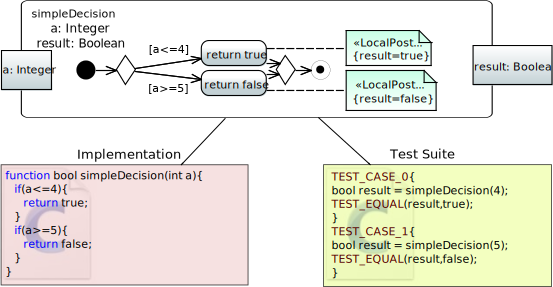
\includegraphics[width=\textwidth]{../Thesis/pics/BasicExamplesSimpleDecision.pdf}
\end{frame}

\begin{frame}
\frametitle{Expressiveness and Complexity of Constraint Languages}
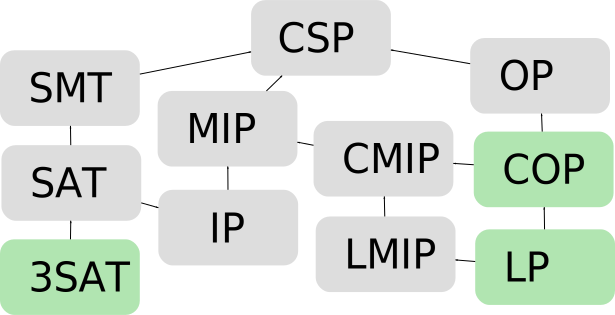
\includegraphics[width=\textwidth]{pics/ProblemLatice.pdf}
\end{frame}

\subsection{Overview}
\begin{frame}
\frametitle{Overview}
\begin{block}{Algorithm}
\begin{description}
\item[Test Model:] UML activity diagram with embedded OCL constraints modelling an operation/function.
\item[Symbolic Execution:] Control flow paths within the activity diagram are converted into a constraint satisfaction problem.
\item[Constraint Solving:] A variety of state--of--the--art constraint solvers are used via AMPL to generate test data.
%\item[Early Infeasible Path Elimination:] Control flow path search is guided by constraint solver.
%\item[Boundary Value Analysis:] Constraint solvers support constrained optimisation out of the box.
\end{description}
\end{block}
\begin{block}{Results}
\begin{description}
\item[Mutation Tests:] Extremly high mutation scores for demo models.
\item[Experimental Runtime Measurements:] Experimental parameter tweaking for test data generation algorithm has been performed.
%\item[Language Independent:] Test model and test cases are stored as an instance of intermediate meta models
\end{description}
\end{block}
\end{frame}


\section{The Algorithm}
% \subsection{Overview}
% \begin{frame}
% \frametitle{Overview of the Algorithm}
% \begin{block}{}
% Map UML/OCL to simplified intermediate representation.
% \end{block}
% \begin{block}{}
% Transform activity diagram into an AMPL model.
% \end{block}
% \begin{block}{}
% Find control flow paths using depth first search with early infeasible path elimination.
% \end{block}
% \begin{block}{}
% Solve constraint satisfaction problem for each control flow path.
% \end{block}
% \begin{block}{}
% Output test cases as C++ unit tests using the Boost test library.
% \end{block}
% \end{frame}

\subsection{AMPL Modelling}
\begin{frame}
\frametitle{AMPL Modelling \cite{AMPL}}
\begin{itemize}
  \item Represent activity diagram in a form that is understood by constraint solvers.
  \item Control flow path is specified as AMPL data.
  \item Solution of an AMPL program is a sequence of variable assignments.
\end{itemize}
\end{frame}

\begin{frame}[fragile]
\frametitle{Basic Example}
\begin{columns}
 \column{.39\textwidth} \ 
	\begin{block}{Activity Diagram} 
	\def\svgwidth{\textwidth}
	\scriptsize
	\import{pics/}{BasicExamples.pdf_tex}
	\end{block} 
\column{.56\textwidth} \ 
	\begin{block}{AMPL Model} 
		\begin{lstlisting}[basicstyle=\ttfamily\scriptsize,language=ampl]
param l; #Pathlength

# Variables (Property or Parameter)
var x{0..l} : integer := 1;
var y : integer := 1;

# Postconditions
set t within {0..l} default {};
s.t. t_post0{i in t} : (y)=(x[i-1]);
s.t. t_post1{i in t} : (x[i])=(x[i-1]);
set e within {0..l} default {};
s.t. e_post0{i in e} : (y)=(x[i-1]-100);
s.t. e_post0{i in e} : (x[i])=(x[i-1]);

# Guards
set d2e within {0..l} default {};
s.t. d2e_g{i in d2e} : (x[i])>=(6.0);
set d2t within {0..l} default {};
s.t. d2t_g{i in d2t} : (x[i])<=(5.0);
\end{lstlisting}
	\end{block} 
\end{columns}
\end{frame}

% \begin{frame}[fragile]
% \frametitle{AMPL Modelling}
% 	\begin{block}{Specify Path} 
% 		\begin{lstlisting}[basicstyle=\ttfamily\small,language=ampl]
% param l := 1;
% set d2f:= 0; # guard 
% set f:= 1; # post condition
% 		\end{lstlisting}
% 	\end{block} 
% 	\begin{block}{Result} 
% 		\begin{lstlisting}[basicstyle=\ttfamily\small]
% Solution determined by presolve.
% a = 5
% return = 0
% 		\end{lstlisting}
% 	\end{block}
% \end{frame}

\subsection{Early Infeasible Path Elimination}
\begin{frame}
\frametitle{Early Infeasible Path Elimination}
	\begin{columns}[c]
		\column[c]{0.4\textwidth}
			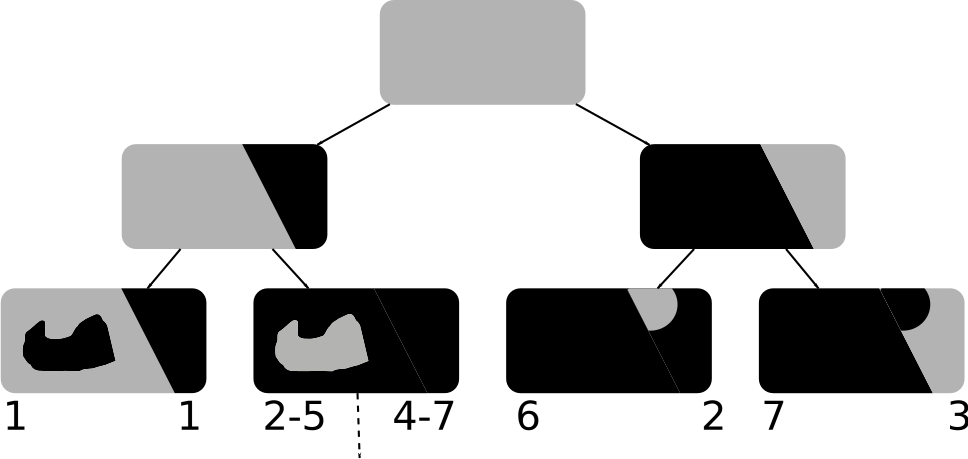
\includegraphics[width=\textwidth]{./pics/VennTree.pdf}
		\column{0.6\textwidth}
				\begin{itemize}
					\item Determine test scenarios fulfilling model structure based coverage criteria efficiently.
					\item To ensure termination activity diagram is unrolled up to a maximum path length.
					\item unchecked steps provide trade--of between early infeasible path elimination and unnecessary overhead.
				\end{itemize}
	\end{columns}
\end{frame}
%TODO
\subsection{Boundary Value Analysis}
\begin{frame}
\frametitle{Boundary Value Analysis}
	\begin{itemize}
		\item For a certain test scenario get the test data most likely to trigger an error.
		\item State–of–the–art constraint solver generates test input and the oracle value from the AMPL program.
		\item Boundary value analysis is possible by adding an objective
function to the AMPL model.
	\end{itemize}
\end{frame}
%ToDo

\section{Evaluation}
\subsection{Example Model}

\begin{frame}
\frametitle{Exploding Tyres (mixed integer non linear)}
% \def\svgwidth{\textwidth}
% \scriptsize
% \input{./pics/TriangleClasificator.pdf_tex}
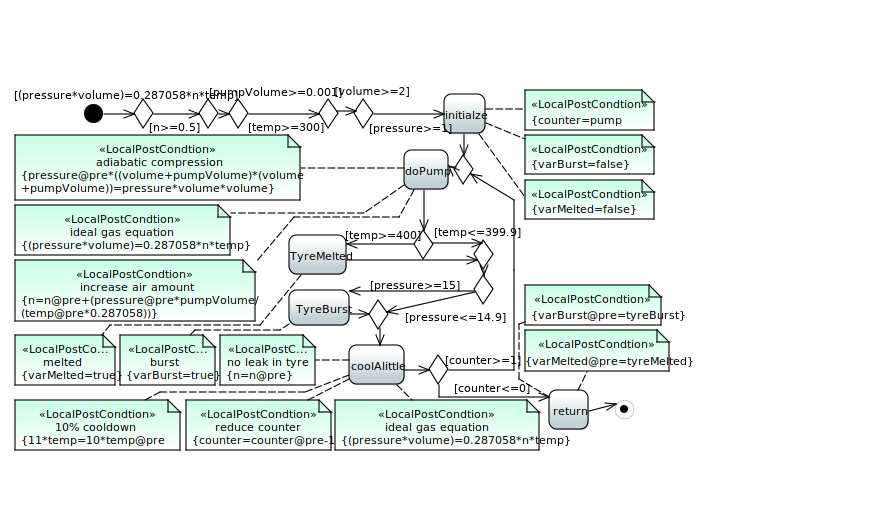
\includegraphics[width=\textwidth]{./pics/TyrePumpModel.pdf}
\end{frame}
\begin{frame}
\frametitle{Runtime with Different Solver Time Limits}
\begin{tikzpicture}
\begin{axis}[
width=0.498\textwidth,
height=7.5cm,
legend style={legend columns=1,at={(0.02,0.98)},anchor=north west},
% legend to name=myLegend,
ylabel={time $[s]$},
xlabel={maximum path length},
yticklabels={{0},{$0.1$},{$1$},{$10$},{$100$},{$10^3$},{$10^4$},{$10^5$}},
extra y ticks={3.6e12,2.592e14},
extra y tick labels={{1h},{3d}},
extra tick style={
        major grid style=black,
        tick align=outside,
        tick style=black
    },
minor x tick num=1,
ymajorgrids=true,
yminorgrids=true,
xmajorgrids=true,
xminorgrids=true,
ymode=log,
xmin=5,
xmax=75,
]
\addplot[blue,no markers] table[x=PATHSEARCH_MAX_PATHLENGTH,y=time(ns)]{../Thesis/Experiment-DATA/ExplodingTyres_10min.csv};
\addlegendentry{10min};
\addplot[red,no markers] table[x=PATHSEARCH_MAX_PATHLENGTH,y=time(ns)]{../Thesis/Experiment-DATA/ExplodingTyres_20sec.csv};
\addlegendentry{20sec};
\addplot[green,no markers] table[x=PATHSEARCH_MAX_PATHLENGTH,y=time(ns)]{../Thesis/Experiment-DATA/ExplodingTyres_5sec.csv};
\addlegendentry{5sec};
% \addplot[dash pattern=on 7pt off 3pt,no markers] table[x=PATHSEARCH_MAX_PATHLENGTH,y=time(ns)]{../Thesis/Experiment-DATA/ExplodingTyres_10s.csv};
% \addlegendentry{10sec};
% \addplot[loosely dashed,no markers] table[x=PATHSEARCH_MAX_PATHLENGTH,y=time(ns)]{../Thesis/Experiment-DATA/ExplodingTyres_60sec.csv};
% \addlegendentry{60sec};
% \addplot[solid,no markers] table[x=PATHSEARCH_MAX_PATHLENGTH,y=time(ns)]{../Thesis/Experiment-DATA/ExplodingTyres_2h.csv};
% \addlegendentry{2h};
\end{axis}
\end{tikzpicture}%
\begin{tikzpicture}
\begin{axis}[
width=0.498\textwidth,
height=7.5cm,
xlabel={maximum path length},
ylabel={number of test cases found},
minor x tick num=1,
minor y tick num=4,
ymajorgrids=true,
yminorgrids=true,
xmajorgrids=true,
xminorgrids=true,
xmin=35,
xmax=75,
]
\addplot[green,no markers] table[x=PATHSEARCH_MAX_PATHLENGTH,y=PathsFound]{../Thesis/Experiment-DATA/ExplodingTyres_5sec.csv};
%\addlegendentry{5sec};
% \addplot[dash pattern=on 7pt off 3pt,no markers] table[x=PATHSEARCH_MAX_PATHLENGTH,y=PathsFound]{Experiment-DATA/ExplodingTyres_10s.csv};
%\addlegendentry{10sec};
\addplot[red,no markers] table[x=PATHSEARCH_MAX_PATHLENGTH,y=PathsFound]{../Thesis/Experiment-DATA/ExplodingTyres_20sec.csv};
%\addlegendentry{20sec};
% \addplot[loosely dashed,no markers] table[x=PATHSEARCH_MAX_PATHLENGTH,y=PathsFound]{Experiment-DATA/ExplodingTyres_60sec.csv};
%\addlegendentry{60sec};
\addplot[blue,no markers] table[x=PATHSEARCH_MAX_PATHLENGTH,y=PathsFound]{../Thesis/Experiment-DATA/ExplodingTyres_10min.csv};
%\addlegendentry{10min};
\end{axis}
\end{tikzpicture}
\end{frame}
\begin{frame}
\frametitle{Mutation Testing the Example Model}
\begin{table}[htb]%
\begin{tabular*}{\textwidth}{@{}l@{\extracolsep{\fill}}*4r}
maximum path length     & 20      & 30      & 40        & 50\\%
\hline%
number of test cases    & 4       & 18      & 47        & 97 \\%
killed mutants          & 553     & 569     & 570       & 573 \\%
alive mutants           & 20      & 4       &  3        & 0 \\%
\hline%
mutation score          & 96.5\%  & 99.3\%  & 99.5\%    & 100\% \\%
\hline%
\end{tabular*}
\label{tab:MutationTesting}%
\end{table}
\end{frame}


\subsection{Case Study}
\begin{frame}
\frametitle{Industrial Case Study (mixed integer linear)}
\begin{itemize}
  \item The Original Model
\begin{itemize}
  \item Activity diagram consists of 21 \UMLType{Action}s, 24 \UMLType{ControlNode}s and two nested \UMLType{LoopNode}s
  \item C code snippets are embedded
\end{itemize}
  \item Manual Adaptations
  \begin{itemize}
  \item All variables and C structs are represented by several \UMLType{Property} elements
  \item OCL constraints are deduced with an educated guess from the embedded C code snippets
  \item Hierarchical \UMLType{LoopNode}s are flattened
\end{itemize}
\end{itemize}
\begin{block}{}
The resulting constraint satisfaction problem is a mixed integer linear program
\end{block}
\end{frame}

\begin{frame}
\frametitle{Runtime Depending on the Unchecked Steps}
\begin{tikzpicture}
\begin{axis}[
width=0.6\textwidth,
height=7.5cm,
legend style={legend columns=1,at={(1.02,0.98)},anchor=north west},
xlabel={unchecked steps},
xmax=15,
ylabel={time $[s]$},
yticklabels={{$1$},{$10$},{$100$},{$10^3$},{$10^4$},{$10^5$}},
extra y ticks={3.6e12,2.592e14},
extra y tick labels={{1h},{3d}},
extra tick style={
        major grid style=black,
        tick align=outside,
        tick style=black
    },
minor x tick num=1,
ymajorgrids=true,
yminorgrids=true,
xmajorgrids=true,
xminorgrids=true,
ymode=log,
]
\addlegendimage{empty legend}
\addlegendentry{maximum path length}
\addplot[densely dashed, blue] table[x=PATHSEARCH_UNCHECKED_STEPS,y=time(ns)]{../Thesis/Experiment-DATA/CaseStudyUncheckedSteps90.csv};
\addlegendentry{90};
\addplot[densely dashed, green] table[x=PATHSEARCH_UNCHECKED_STEPS,y=time(ns)]{../Thesis/Experiment-DATA/CaseStudyUncheckedSteps80.csv};
\addlegendentry{80};
\addplot[densely dashed, red] table[x=PATHSEARCH_UNCHECKED_STEPS,y=time(ns);]{../Thesis/Experiment-DATA/CaseStudyUncheckedSteps70.csv};
\addlegendentry{70};
\addplot[blue] table[x=PATHSEARCH_UNCHECKED_STEPS,y=time(ns);]{../Thesis/Experiment-DATA/CaseStudyUncheckedSteps60.csv};
\addlegendentry{60};
\addplot[green] table[x=PATHSEARCH_UNCHECKED_STEPS,y=time(ns)]{../Thesis/Experiment-DATA/CaseStudyUncheckedSteps50.csv};
\addlegendentry{50};
\addplot[red] table[x=PATHSEARCH_UNCHECKED_STEPS,y={time(ns)}]{../Thesis/Experiment-DATA/CaseStudyUncheckedSteps40.csv};
\addlegendentry{40};
\end{axis}
\end{tikzpicture}
\end{frame}

\begin{frame}
\frametitle{Runtime for Different Solvers}
\begin{tikzpicture}
\begin{axis}[
width=0.59\textwidth,
height=7.5cm,
%legend columns=-1,
%legend to name=solvers,
legend style={at={(0.02,0.98)},anchor=north west},
xlabel={maximum path length},
ylabel={time $[s]$},
yticklabels={0,{$1$},{$10$},{$100$},{$10^3$},{$10^4$},{$10^5$}},
extra y ticks={3.6e12,2.592e14},
extra y tick labels={{1h},{3d}},
extra tick style={
        major grid style=black,
        tick align=outside,
        tick style=black
    },
minor x tick num=1,
xmin=15,
xmax=115,
ymax=1e14,
ymajorgrids=true,
yminorgrids=true,
xmajorgrids=true,
xminorgrids=true,
ymode=log,
]
\addplot[green] table[x=PATHSEARCH_MAX_PATHLENGTH,y=time(ns)] {../Thesis/Experiment-DATA/CaseStudyRuntimeCplex.csv};
\addlegendentry{Cplex};
\addplot[blue] table[x=PATHSEARCH_MAX_PATHLENGTH,y=time(ns)] {../Thesis/Experiment-DATA/CaseStudyRuntimeLPSolve.csv};
\addlegendentry{LPsolve};
\addplot[orange] table[x=PATHSEARCH_MAX_PATHLENGTH,y=time(ns)] {../Thesis/Experiment-DATA/CaseStudyRuntimeCouenne.csv};
\addlegendentry{Couenne};
\addplot[red] table[x=PATHSEARCH_MAX_PATHLENGTH,y=time(ns)] {../Thesis/Experiment-DATA/CaseStudyRuntimeGecode.csv};
\addlegendentry{GeCoDE};
\addplot[dashed] expression[no markers, domain=30:110]{2e7*1.12^(x)} node[pos=0.5,sloped,fill=white, below, opacity=1,text opacity=1] {$1.12 ^ {x}$} ;
\end{axis}
\end{tikzpicture}%
\begin{tikzpicture}
\begin{axis}[
width=0.39\textwidth,
height=7.5cm,
ylabel={number of test cases},
xlabel={maximum path length},
minor x tick num=4,
ymajorgrids=true,
yminorgrids=true,
xmajorgrids=true,
xminorgrids=true,
ymode=log,
]
\addplot[blue] table[x=PATHSEARCH_MAX_PATHLENGTH,y=PathsFound]{../Thesis/Experiment-DATA/CaseStudyRuntimeLPSolve.csv};
\addplot[color=black, style=dashed] expression[no markers, domain=30:100]{1.1 ^ (x)} 
node[pos=0.5,sloped,fill=white, below, opacity=1,text opacity=1] {$1.1 ^ {x}$}
;
\end{axis}
\end{tikzpicture}
\end{frame}

\begin{frame}
\frametitle{Runtime with and without Boundary Value Analysis}
\begin{tikzpicture}
\begin{axis}[
width=\textwidth,
height=7.5cm,
%title={Influence of boundary value analysis},
legend style={at={(0.02,0.98)},anchor=north west},
ylabel={time $[s]$},
xlabel={maximum path length},
%ytick={1e8,1e10,1e12,1e14},
yticklabels={0,{1},{10},{100},{$10^3$},{$10^4$},{$10^5$}},
extra y ticks={3.6e12,2.592e14},
extra y tick labels={{1h},{3d}},
extra tick style={
        major grid style=black,
        tick align=outside,
        tick style=black
    },
ymajorgrids=true,
yminorgrids=true,
xmajorgrids=true,
xminorgrids=true,
ymode=log,
]
\addplot[blue] table[x=PATHSEARCH_MAX_PATHLENGTH,y=time(ns)]{../Thesis/Experiment-DATA/CaseStudyRuntimeBoundaryValues.csv};
\addlegendentry{with};
\addplot[red] table[x=PATHSEARCH_MAX_PATHLENGTH,y=time(ns)]{../Thesis/Experiment-DATA/CaseStudyRuntimeNoBoundaryValues.csv};
\addlegendentry{without}
\end{axis}
\end{tikzpicture}%
\end{frame}

% \begin{frame}
% \frametitle{Experiments Summary}
% \begin{itemize}
%   \item Runtime measurements varying solvers and parameters
%   \item Mutation testing
%   \item Runtime grows exponentially with maximum path length
%   \item Early infeasible path recognition drastically reduces the runtime
%   \item Sub--optimal execution plans are detected as error
% \end{itemize}
% \end{frame}

\section{Summary \& Outlook}
\subsection{Summary}
\begin{frame}
\frametitle{Summary}
\begin{itemize}
  \item Current constraint solvers can efficiently generate test data for industry scale applications.
  \item Mixed integer linear programming can be handled highly efficient.
  \item Test generation for models with mixed integer non-linear constraints is possible but time consuming.
  \item Early infeasible path recognition with 2 unchecked steps drastically reduces the runtime.
  \item Boundary Value Analysis can be performed with tiny additional effort.
  \item A fully working proof-of-concept tool is available at \href{http://parteg.sourceforge.net/}{http://parteg.sourceforge.net/}.
\end{itemize}
\end{frame}

\subsection{Outlook}
\begin{frame}
\frametitle{Outlook}
\begin{itemize}
  \item Add support for further UML/OCL modelling elements and features e.g. \UMLType{CallBehaviourAction} and complex data types.
  \item Add support for other output languages and test frameworks.
  \item Reuse test goal management from ParTeG to support feasible coverage criteria instead of all control flow paths.~\cite{ParTeG}
\end{itemize}
\end{frame}

\section{Demonstration}
\begin{frame}
\begin{block}{}
\begin{center}
\Huge{Demonstration}
\end{center}
\end{block}
\end{frame}



% \begin{frame}
% \begin{block}{Thank you!}
% \begin{center}
% \Huge{Questions?}
% \end{center}
% \end{block}
% \end{frame}
\frametitle{Bibliography}
\bibliographystyle{IEEEtran}
%\bibliographystyle{plain}
\bibliography{../Thesis/bibtex}
\end{document}
